\chapter{Implementation}
The implementation is based on ROS (Robot Operating System), which provides a a communication infrastructure for a project, which allows multiple programs to communicate between each other. 

Each program runs in individual threads, called nodes, such that their timing is independent from each other, except for hardware limitations. This allows each node to run in parallel in multiple threads while still being able to share data between them.

The data sharing is done through topics, onto which the nodes can publish and subscribe to. Each topic contains the data stored in a predefined data structure, specified as a message, such that each node publishes or reads data of the same type.

A diagram of the particular implementation, including nodes and topics can be seen in \autoref{fig:diagramROS}.

\begin{figure}[H]
    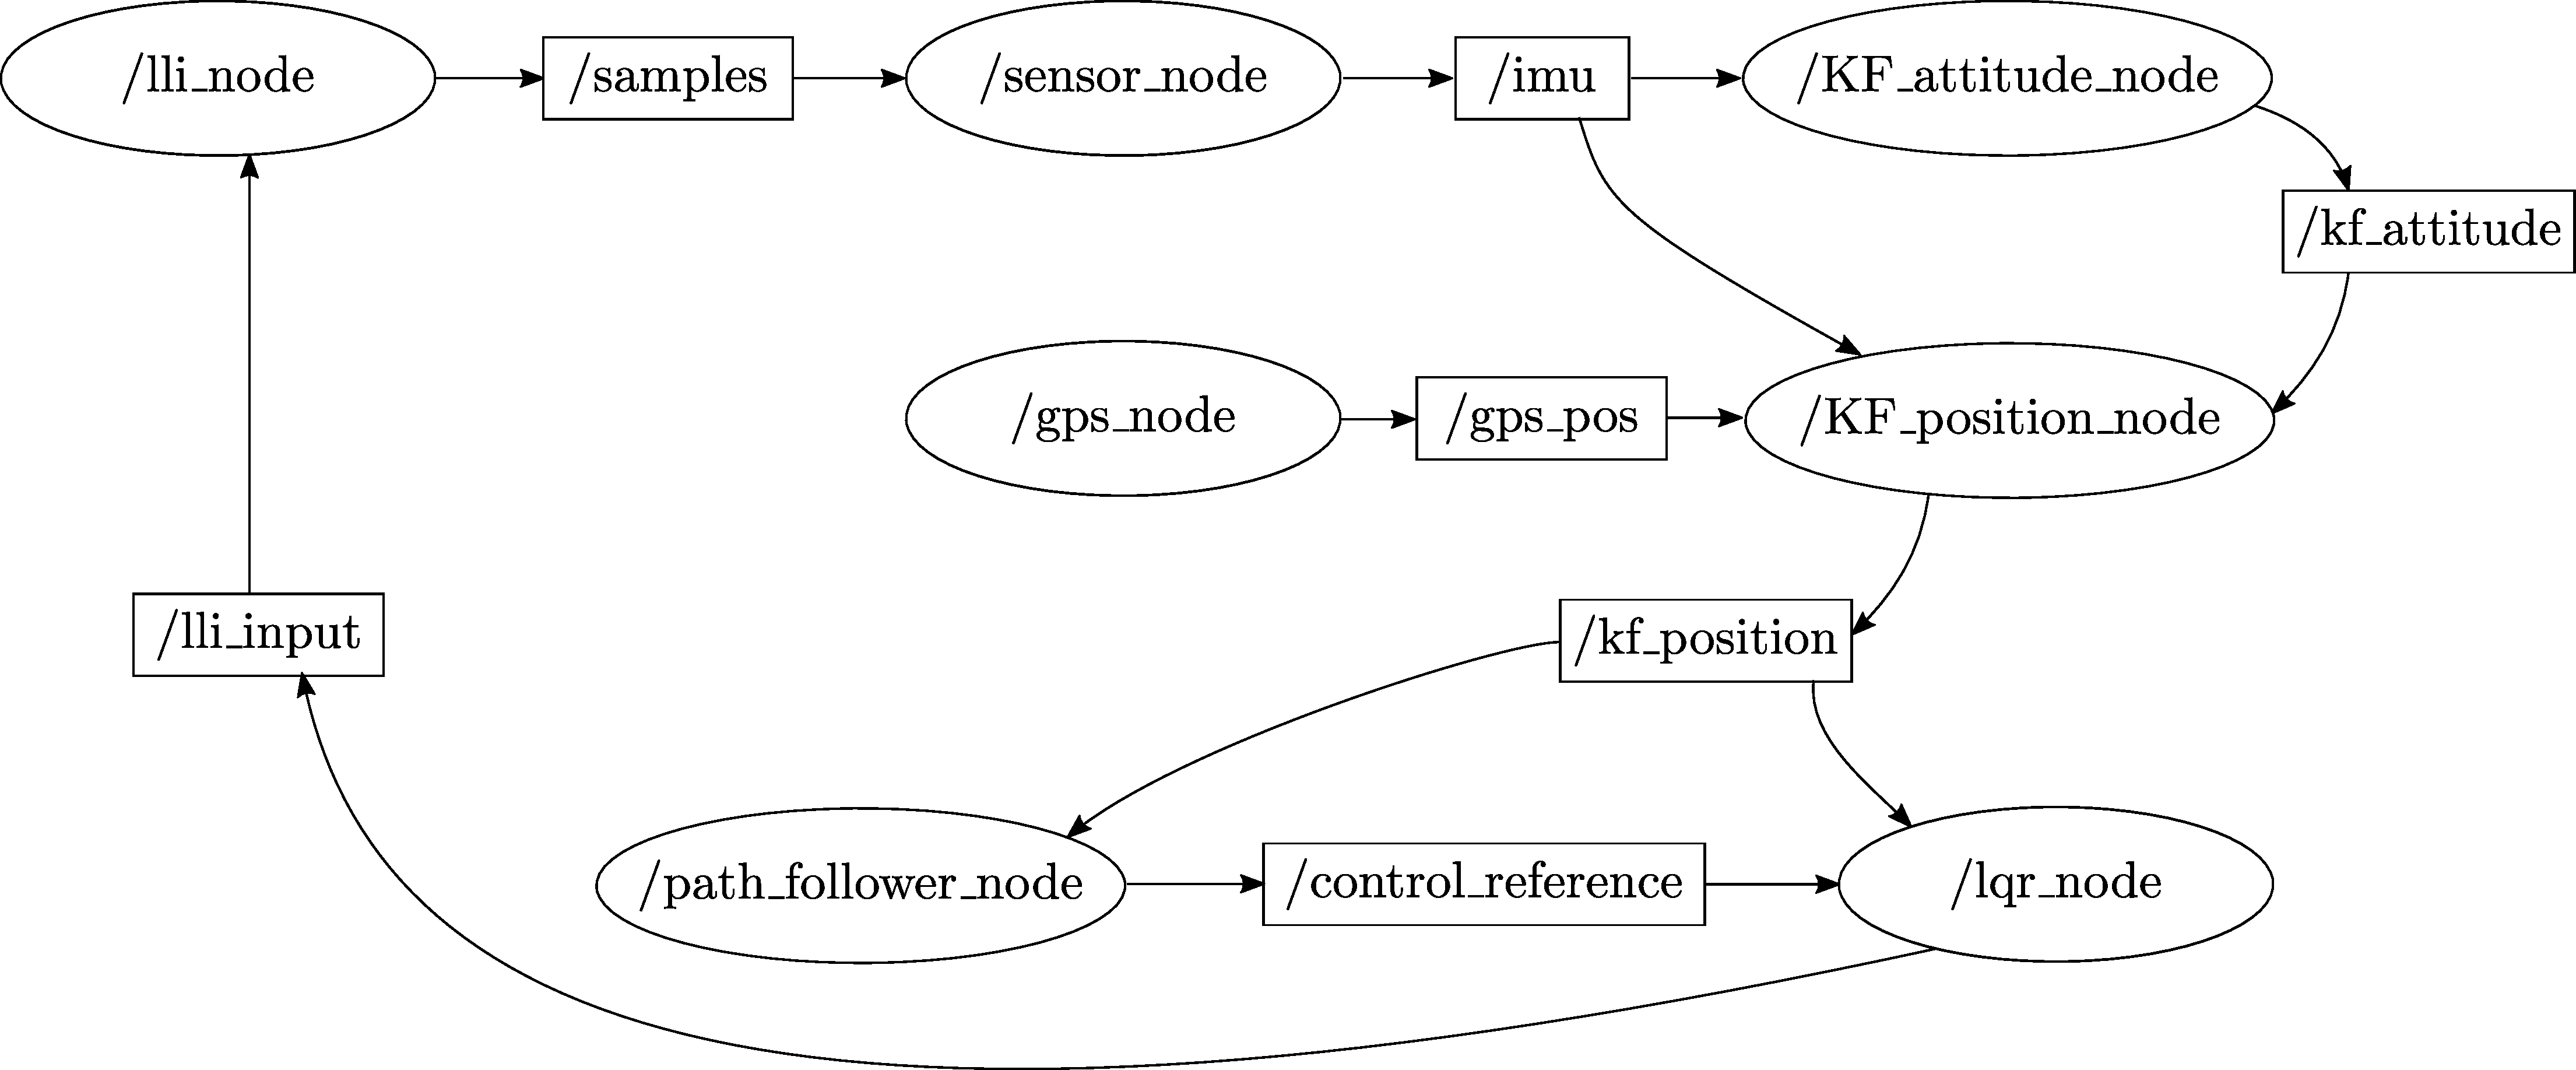
\includegraphics[width=0.7\textwidth]{figures/diagramROS}
    \caption{Diagram of the implementation in ROS, which includes the relations between nodes and topics.}
    \label{fig:diagramROS}
\end{figure}

A more detailed explanation of the functionality of each node and the data contained in each topic is presented in this chapter.


%
% 
%\subsection{System overview}
%The system consists of two subsystems, a Low-Level-Interface (LLI) and a High-Level-Interface (HLI). 
%The LLI is a hardware interface, responsible for reading all the sensors and sending control signals to the motors.
%The HLI contains the sensor fusion, and the controllers, as well as a interface to the operator. 
%The LLI is designed and implemented in a previous project, and wont be described in detail, which is also applicable of the sensor fusion from the HLI.\fxnote{Ensure this is also true in the future (:}
%
%\subsection{Route following node}
%The route following uses waypoints together with position data to generate a reference for the low level controller. 
%The method described in section\fxnote{Ref to section describing Route following node} describes the line between two waypoints as an affine linear line.  
%This description have the issue of having singularity when describing vertical lines, making the slope infinite.  
%This issue is avoided in the implemented algorithm by using a different description of a line. 
%The description uses polar coordinates to describe the line going from the center of the boat and hitting the line between waypoints perpendicularly.
%\autoref{fig:line_polar} illustrates how this  description is used. 
%$W_{prev}$ and $W_{next}$ is the two waypoints, r is the distance from the boat to the line between them and $\theta$ is the angle.
%\begin{figure}[H]
%  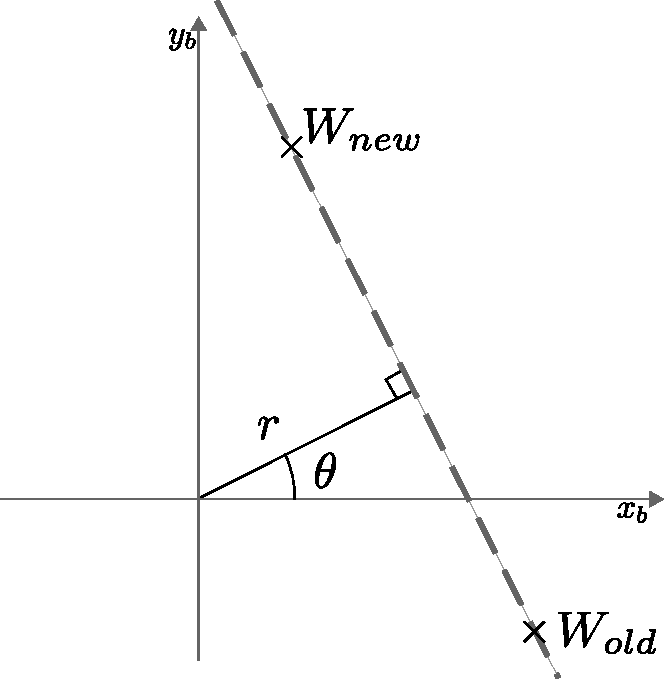
\includegraphics[width=0.5\textwidth]{figures/waypoint_line}
%  \caption{Illustration of line specification}
%  \label{fig:line_polar}
%\end{figure}
%This description requires the transformation of the waypoints from the inertial frame to the boat frame.
%The angle between the waypoints can be computed by:
%\begin{flalign}
%	\theta = atan\frac{\Delta y}{\Delta x}
%\end{flalign}
%\begin{where}
%  \va{\Delta x}{is the difference in x between the two waypoints}{m}
%  \va{\Delta y}{is the difference in y between the two waypoints}{m}
%\end{where}
%
%The radius between the boat and the waypoint line can then be computed by.
%\begin{flalign}
%	r = x\sin{\theta} + y\cos{\theta}
%\end{flalign}

